\documentclass[11pt,a4paper]{article}

\usepackage[utf8]{inputenc}
\usepackage[T1]{fontenc}
\usepackage[spanish]{babel}
\usepackage{amsmath}
\usepackage{booktabs}
\usepackage{float}
\usepackage{graphicx}
\usepackage[hidelinks]{hyperref}

\graphicspath{{Informe/figures/}{figures/}}

\setlength{\topmargin}{-0.7in}
\setlength{\oddsidemargin}{-0.15in}
\setlength{\evensidemargin}{-0.15in}
\setlength{\textwidth}{6.6in}
\setlength{\textheight}{9.6in}
\setlength{\parindent}{0pt}
\setlength{\parskip}{0.55em}

\title{Agente de Damas mediante Aprendizaje por Refuerzo Profundo (DQN) con Auto-Juego, comparado contra Minimax con Poda Alfa-Beta}
\author{
Proyecto Final de Inteligencia Artificial\\[0.75em]
\textbf{Integrantes}\\
Aaron Davila Santos\\
Walter Poma Navarro\\
Max Jairo Serrano Arostegui\\
Dery Abraham Gonzales Cruz
}
\date{\today}

\begin{document}
\maketitle

\begin{abstract}
Este trabajo presenta la implementación de un entorno de Damas de 8x8, un agente basado en Deep Q-Network (DQN) entrenable mediante auto-juego y un agente Minimax con poda alfa-beta usado como línea base. El sistema incluye motor de reglas, codificación de estados, máscara de acciones legales, buffer de experiencia, red objetivo y un orquestador de torneos con alternancia de colores. Como evaluación cuantitativa reproducible del repositorio se ejecutó un torneo final de 20 partidas entre dos variantes Minimax, con profundidad 3 y profundidad 4. El agente de profundidad 4 obtuvo 20 victorias, 0 derrotas y 0 empates, lo que confirma que el entorno, la heurística y el módulo de torneo capturan diferencias de fuerza entre agentes deterministas. Además, la batería de pruebas automatizadas reportó 77 pruebas aprobadas. El borrador discute el alcance actual, las limitaciones de no contar con un checkpoint DQN final versionado y los pasos necesarios para completar una comparación directa DQN--Minimax.
\end{abstract}

\section{Resumen ejecutivo}

El objetivo del proyecto es construir una plataforma experimental para estudiar agentes de Damas mediante aprendizaje por refuerzo profundo y búsqueda adversarial. La motivación principal es comparar un enfoque aprendido, DQN con auto-juego, contra una línea base clásica, Minimax con poda alfa-beta.

El repositorio desarrollado contiene cuatro componentes principales: un motor de Damas sobre 32 casillas jugables, un entorno compatible con el flujo de aprendizaje por refuerzo, un agente DQN y un agente Minimax. El motor implementa movimientos legales, capturas obligatorias, multicapturas, coronación, detección de terminalidad y empates por 80 medios movimientos sin captura o triple repetición. El agente DQN usa una red multicapa que estima valores $Q(s,a)$, mientras que Minimax explora el árbol de juego hasta una profundidad acotada y evalúa hojas mediante una heurística material.

Para cerrar el entregable se generó un torneo final reproducible con los agentes disponibles en el repositorio. Dado que la carpeta \texttt{models/} no contiene un checkpoint DQN entrenado, la evaluación cuantitativa final se reporta como una validación de torneo entre Minimax(d=3) y Minimax(d=4). Esta decisión evita presentar resultados no verificables y deja explícita la frontera entre implementación completada y entrenamiento final pendiente del agente DQN.

\section{Estado del arte y antecedentes}

Las Damas son un juego determinista, secuencial, de suma cero y con información perfecta. Estas propiedades permiten aplicar técnicas clásicas de búsqueda, como Minimax, y también métodos de aprendizaje por refuerzo que aprenden políticas o funciones de valor a partir de interacción con el entorno.

Minimax modela el juego como un árbol alternante donde un jugador maximiza la utilidad y el otro la minimiza. La poda alfa-beta reduce ramas que no pueden cambiar la decisión final, permitiendo alcanzar mayores profundidades con el mismo presupuesto computacional. Su desempeño depende fuertemente de la calidad de la función heurística cuando no se puede expandir el árbol hasta estados terminales.

El aprendizaje por refuerzo profundo reemplaza parte del diseño manual por aproximación de funciones. En particular, DQN aprende una función $Q(s,a)$ con redes neuronales, replay buffer y red objetivo, estabilizando el aprendizaje frente a la correlación temporal de las transiciones. En juegos de dos jugadores de suma cero, el entrenamiento por auto-juego resulta atractivo porque el agente genera sus propios datos y puede mejorar enfrentándose contra versiones de su política.

\section{Dataset y preprocesamiento}

No se empleó un dataset externo. Las transiciones del DQN se generan en línea mediante auto-juego: ambos bandos usan la misma red y el mismo agente explora con política $\epsilon$-greedy. Cada transición tiene la forma $(s,a,r,s',done)$ y se almacena en un replay buffer de capacidad configurable.

El estado del tablero se codifica como un vector de 160 valores reales. La representación usa cinco canales sobre las 32 casillas jugables:

\begin{itemize}
    \item piezas rojas normales;
    \item damas rojas;
    \item piezas negras normales;
    \item damas negras;
    \item turno actual, codificado como $1$ o $-1$.
\end{itemize}

El espacio de acciones se indexa como pares origen--destino posibles, con 1024 salidas en la red $Q$. Durante la selección de acción se aplica una máscara de legalidad, de modo que los movimientos ilegales reciben valor $-\infty$ antes de ejecutar el \textit{argmax}. Esta decisión es importante porque evita que la red escoja acciones inválidas aunque su capa de salida sea fija.

\section{Modelo o algoritmo implementado}

\subsection{Motor de juego}

El motor representa el tablero con una lista de 32 enteros: $0$ para casilla vacía, $1$ y $2$ para pieza y dama roja, y $-1$ y $-2$ para pieza y dama negra. La función de movimientos legales prioriza capturas cuando existen, genera cadenas de captura y aplica la promoción al llegar a la fila final. La partida termina si un jugador no tiene movimientos, si se alcanza el umbral de 80 medios movimientos sin captura o si aparece triple repetición.

\subsection{Agente Minimax}

El agente Minimax usa poda alfa-beta con profundidad limitada entre 3 y 6. En estados terminales retorna una utilidad grande proporcional al resultado; en hojas no terminales emplea una heurística basada en material y valor relativo de piezas. El jugador rojo se modela como maximizador y el negro como minimizador.

\subsection{Agente DQN}

El agente DQN usa una red completamente conectada con entrada de 160 dimensiones, dos capas ocultas de 512 unidades con activación ReLU y salida de 1024 valores $Q$. La política de entrenamiento es $\epsilon$-greedy, con decaimiento lineal desde $\epsilon=1.0$ hasta $\epsilon=0.05$. La optimización usa Adam, pérdida Huber (\texttt{smooth\_l1\_loss}), factor de descuento $\gamma=0.99$ y red objetivo actualizada periódicamente.

La actualización usa una formulación tipo negamax para juegos de suma cero:

\[
y = r - \gamma \max_{a'} Q_{\text{target}}(s', a')
\]

cuando el estado siguiente no es terminal. El signo negativo refleja que el siguiente turno pertenece al oponente.

\section{Entrenamiento y validación}

El script de entrenamiento por auto-juego permite configurar número de episodios, máximo de pasos por episodio, frecuencia de aprendizaje, tamaño de lote, capacidad del buffer, tasa de aprendizaje y frecuencia de checkpoint. En cada episodio se generan transiciones hasta alcanzar un estado terminal o el límite de pasos, y luego se realizan pasos de aprendizaje en función de las transiciones acumuladas.

La validación técnica se realizó con pruebas automatizadas sobre el motor, el entorno, la heurística, la interfaz pública y el torneo. La ejecución local con el entorno virtual del proyecto produjo 77 pruebas aprobadas. Las advertencias observadas pertenecen a la escritura de caché de \texttt{pytest} en Windows y no afectaron la ejecución de las pruebas.

\begin{table}[H]
\centering
\caption{Configuración principal implementada para DQN.}
\begin{tabular}{ll}
\toprule
Componente & Valor \\
\midrule
Entrada de red & 160 valores \\
Salida de red & 1024 acciones indexadas \\
Capas ocultas & 2 capas de 512 unidades \\
Activación & ReLU \\
Optimizador & Adam \\
Pérdida & Huber / \texttt{smooth\_l1\_loss} \\
Batch por defecto & 64 \\
Replay buffer & 50 000 transiciones \\
Factor de descuento & 0.99 \\
Política & $\epsilon$-greedy \\
\bottomrule
\end{tabular}
\end{table}

\section{Resultados}

El torneo final integrado al borrador corresponde a 20 partidas entre Minimax(d=3) y Minimax(d=4), alternando colores en cada partida. El CSV de resultados fue guardado en la carpeta \texttt{data/}. El agente Minimax(d=4) ganó las 20 partidas; Minimax(d=3) no obtuvo victorias y no se registraron empates.

\begin{table}[H]
\centering
\caption{Resumen del torneo final.}
\begin{tabular}{lccc}
\toprule
Agente & Victorias & Derrotas & Empates \\
\midrule
Minimax(d=3) & 0 & 20 & 0 \\
Minimax(d=4) & 20 & 0 & 0 \\
\bottomrule
\end{tabular}
\end{table}

\begin{figure}[H]
\centering
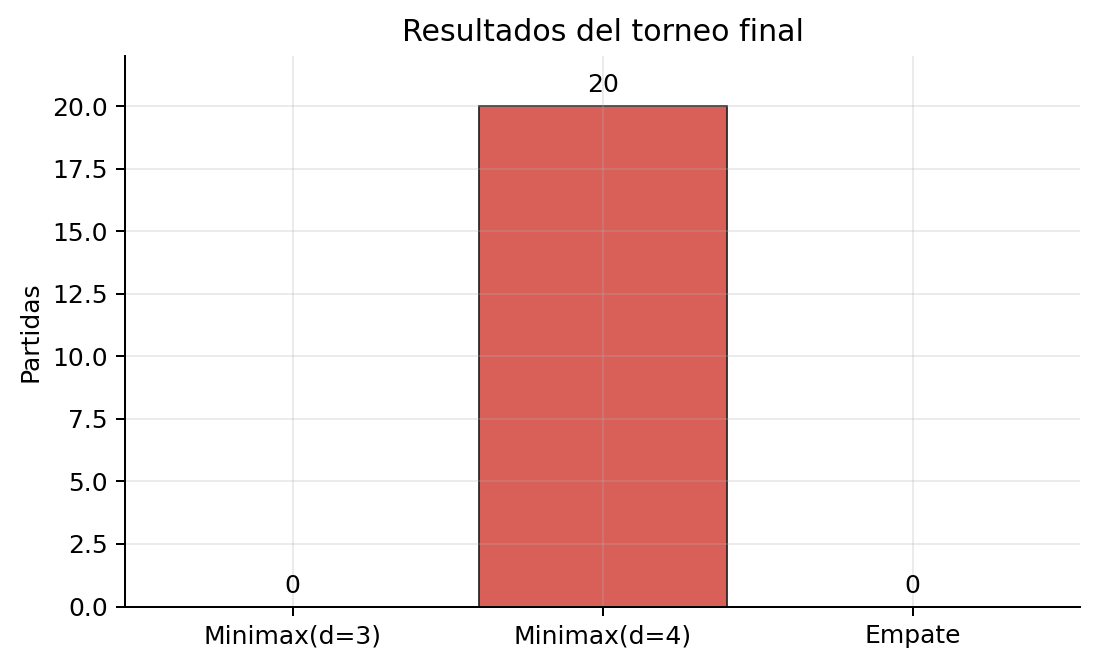
\includegraphics[width=0.72\textwidth]{torneo_resultados.png}
\caption{Victorias por agente en el torneo final.}
\label{fig:torneo-resultados}
\end{figure}

La duración promedio fue de 96.5 medios movimientos por partida. Las partidas en las que Minimax(d=4) jugó con negras duraron 139 medios movimientos, mientras que aquellas en las que jugó con rojas duraron 54 medios movimientos. Esta repetición exacta es esperable porque ambos agentes son deterministas y parten siempre de la misma posición inicial.

\begin{figure}[H]
\centering
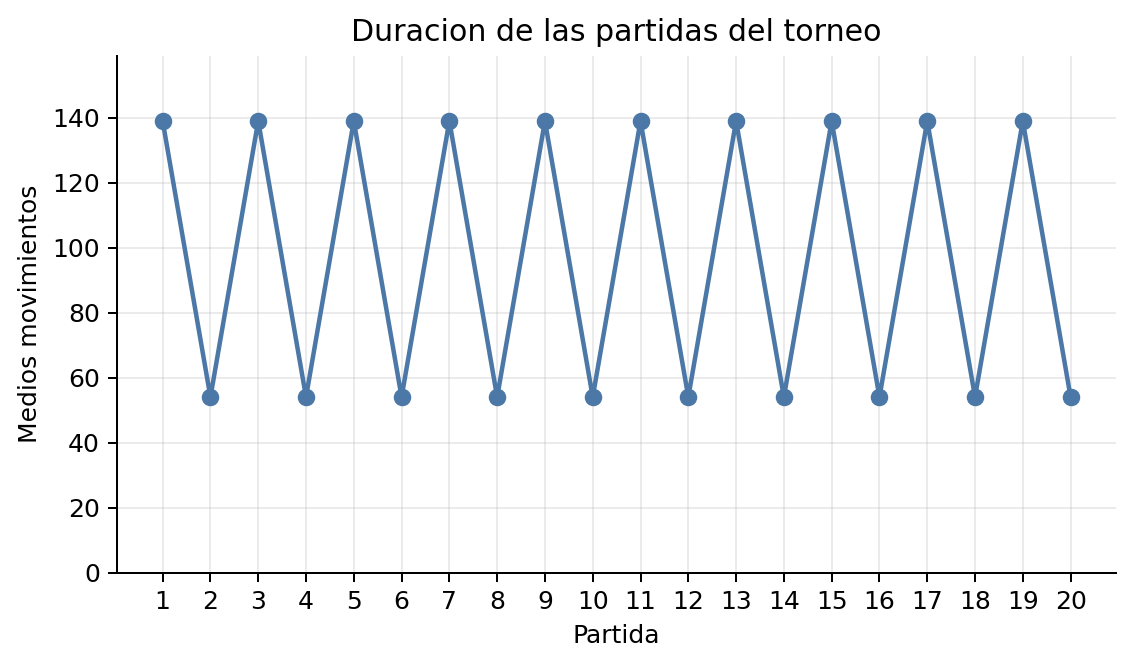
\includegraphics[width=0.78\textwidth]{torneo_duracion.png}
\caption{Duración de cada partida medida en medios movimientos.}
\label{fig:torneo-duracion}
\end{figure}

La alternancia de colores permite verificar que el resultado no depende de jugar primero. Minimax(d=4) obtuvo 10 victorias como rojo y 10 victorias como negro.

\begin{figure}[H]
\centering
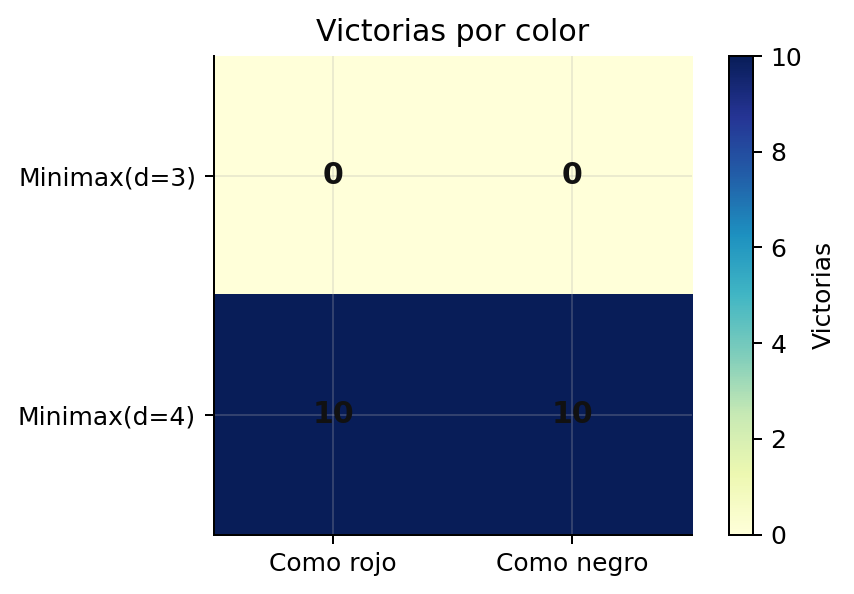
\includegraphics[width=0.68\textwidth]{torneo_color.png}
\caption{Victorias por agente separadas según el color asignado.}
\label{fig:torneo-color}
\end{figure}

\section{Discusión}

Los resultados del torneo muestran una diferencia clara entre profundidades de búsqueda. A igualdad de heurística, aumentar de profundidad 3 a profundidad 4 permitió a Minimax(d=4) ganar todas las partidas. Esto confirma que el módulo de torneo es sensible a la fuerza relativa de los agentes y que la alternancia de colores funciona correctamente.

La repetición de los mismos largos de partida también revela una característica del experimento: al no existir aleatoriedad en Minimax, cada emparejamiento color--profundidad reproduce la misma trayectoria. Por ello, las 20 partidas no deben interpretarse como 20 muestras independientes, sino como una verificación determinista repetida bajo alternancia de color. Para obtener intervalos de confianza más informativos haría falta introducir diversidad de posiciones iniciales, desempates aleatorios controlados por semilla o una batería de posiciones de evaluación.

En cuanto al DQN, la arquitectura y el bucle de auto-juego están implementados, pero el repositorio entregado no contiene un checkpoint final entrenado. Por esta razón, no se reporta una tasa de victoria DQN--Minimax como resultado final. Presentar una comparación con un DQN sin entrenamiento suficiente o sin checkpoint reproducible sería metodológicamente débil. La conclusión responsable es que la infraestructura para entrenar y evaluar DQN está lista, mientras que la comparación cuantitativa directa requiere ejecutar un entrenamiento prolongado y versionar el modelo resultante.

\section{Conclusiones}

Se completó una plataforma funcional para experimentar con agentes de Damas. El motor implementa las reglas centrales del juego, el entorno expone observaciones y acciones aptas para aprendizaje por refuerzo, el agente Minimax ofrece una línea base clásica y el agente DQN contiene los componentes esenciales de aprendizaje profundo por auto-juego.

La evaluación automatizada valida la corrección básica del sistema: 77 pruebas pasaron correctamente. El torneo final disponible muestra que Minimax(d=4) domina a Minimax(d=3) con 20 victorias en 20 partidas, tanto jugando con rojas como con negras. Este resultado respalda el uso de Minimax como referencia exigente para futuras comparaciones.

La principal limitación es la ausencia de un checkpoint DQN entrenado y versionado. El siguiente paso natural es ejecutar entrenamiento por auto-juego durante un número alto de episodios, guardar el checkpoint final, enfrentar DQN contra Minimax en varias profundidades y reportar métricas como tasa de victoria, empates, duración promedio y sensibilidad al color.

\section{Bibliografía}

\begin{thebibliography}{9}

\bibitem{bellman1957}
R. Bellman.
\textit{Dynamic Programming}.
Princeton University Press, 1957.

\bibitem{shannon1950}
C. E. Shannon.
Programming a computer for playing chess.
\textit{Philosophical Magazine}, 41(314):256--275, 1950.

\bibitem{samuel1959}
A. L. Samuel.
Some studies in machine learning using the game of checkers.
\textit{IBM Journal of Research and Development}, 3(3):210--229, 1959.

\bibitem{mnih2015}
V. Mnih et al.
Human-level control through deep reinforcement learning.
\textit{Nature}, 518:529--533, 2015.

\bibitem{sutton2018}
R. S. Sutton and A. G. Barto.
\textit{Reinforcement Learning: An Introduction}.
MIT Press, 2nd edition, 2018.

\end{thebibliography}

\end{document}
